\documentclass[a4paper, 12pt]{article}

\usepackage{hyperref}
\usepackage[warn]{mathtext}
\usepackage[utf8]{inputenc}
\usepackage[T2A]{fontenc}
\usepackage[english,russian]{babel}
\usepackage{multirow}
\usepackage{float}
\restylefloat{table}
\usepackage{amsmath,amsfonts,amssymb,amsthm,mathtools}
\usepackage{indentfirst}
\DeclareSymbolFont{T2Aletters}{T2A}{cmr}{m}{it}
\usepackage{ gensymb }
\mathtoolsset{showonlyrefs=true}
\usepackage{euscript}
\usepackage{mathrsfs}
\usepackage[left=2cm,right=2cm,top=2cm,bottom=2cm]{geometry}
\usepackage{graphicx}
\usepackage{wrapfig}
\usepackage[rgb]{xcolor}
\hypersetup{
colorlinks=true,
urlcolor=blue
}
\usepackage{tikz}

\begin{document}

	\begin{titlepage}
	\begin{center}
		{\large МОСКОВСКИЙ ФИЗИКО-ТЕХНИЧЕСКИЙ ИНСТИТУТ (НАЦИОНАЛЬНЫЙ ИССЛЕДОВАТЕЛЬСКИЙ УНИВЕРСИТЕТ)}
	\end{center}
	\begin{center}
		{\large Физтех-школа прикладной математики и информатики}
	\end{center}
	
	
	\vspace{4.5cm}
	{\huge
		\begin{center}
			{\bf Отчёт о выполнении лабораторной работы 3.4.5}\\
			Петля гистерезиса (динамический метод)
		\end{center}
	}
	\vspace{1cm}
	\begin{center}
		{\large Соболевский Федор Александрович \\
			\vspace{0.2cm}
			Б05-111}
	\end{center}
	\vspace{8cm}
	\begin{center}
		Декабрь 2022
	\end{center}
\end{titlepage}

\section{Аннотация}

В данной работе при помощи электронного осциллографа исследовались предельные петли гистерезиса и начальные кривые намагничивания для нескольких ферромагнитных образцов, были определены магнитные характеристики материалов, чувствительность каналов X и Y осциллографа и постоянная времени $\tau$ интегрирующей ячейки.

\section{Теоретические сведения}

Основные характеристики
ферромагнетиков — их коэрцитивное поле $H_c$, магнитная проницаемость
$\mu$, рассеиваемая в виде тепла при перемагничивании мощность — зависят
от частоты перемагничивающего поля. В данной работе кривые гистерезиса ферромагнитных материалов изучаются в поле частоты $\nu_0 = 50~Гц$
с помощью электронного осциллографа.

\begin{figure}[H]
\begin{center}
    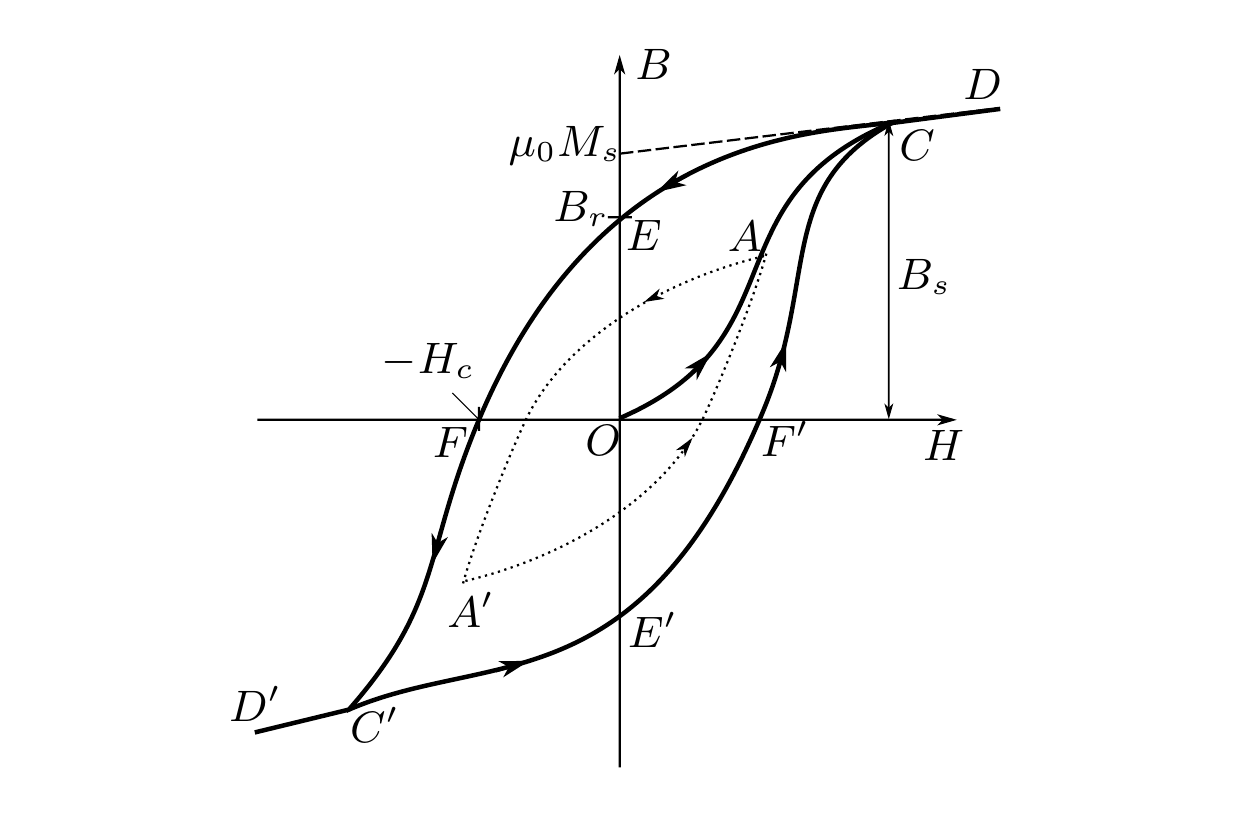
\includegraphics[scale=2]{1.png}
\end{center}
\caption{Петля гистерезиса ферромагнетика}
\label{fig:petlya}
\end{figure}

Магнитная индукция $ B $ и напряжённость поля $ H $ в ферромагнитном материале неоднозначно связаны между собой: индукция зависит
не только от напряжённости, но и от предыстории образца. Связь между $ B $ и $ H $ типичного ферромагнетика иллюстрирует рис.~\ref{fig:petlya}.

Если к ферромагнитному образцу прикладывать переменное внешнее
магнитное поле, то его состояние на плоскости $ B-H $ будет изменяться
по замкнутой кривой — петле гистерезиса. Размер петли определяется
максимальным значением напряжённости $ H $ в цикле (например, петля $ AA' $,
обозначенная пунктиром на рис.~\ref{fig:petlya}). Если амплитуда напряжённости достаточно велика, то образец будет периодически достигать насыщения,
что на рисунке соответствует кривой $ CEFC'E'F'C $ (предельная петля
гистерезиса). Пересечение предельной петли с вертикальной осью соответствует остаточной индукции $B_r$, пересечение с горизонтальной осью
— коэрцитивному полю $H_c$. Крайние точки петель, соответствующие амплитудным значениям $ H $ (например, точка $ A $ на рис.~\ref{fig:petlya}), лежат на начальной кривой намагничивания ($ OAC $).

\subsection{Измерение магнитной индукции}

Магнитную индукцию $ B $ удобно определять с помощью ЭДС, возникающей при изменении магнитного потока $ \Phi $ в катушке, намотанной на образец. Пусть катушка c $ N $ витками плотно охватывает образец сечением $ S $, и индукция $ B $ в образце однородна. Тогда

\begin{equation}
|B|=\frac{1}{SN}\int\mathcal{E} dt.
\label{eq:|B|}
\end{equation}

\begin{wrapfigure}{r}{0.35\linewidth}
	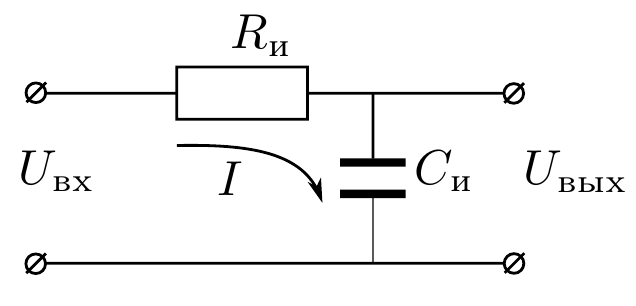
\includegraphics[width=\linewidth]{2.png}
	\caption{Интегрирующая ячейка}
	\label{fig:int}
\end{wrapfigure}

Для интегрирования в работе используется интегрирующая $ RC $-цепочка (рис.~\ref{fig:int}). «Входное» напряжение от источника $U_{\text{вх}}(t)$ подаётся на последовательно соединённые резистор $R_\text{и}$ и конденсатор $C_\text{и}$. <<Выходное>> напряжение $U_{\text{вых}}(t)$ снимается с конденсатора. Предположим, что 1) сопротивление источника мало по сравнению с $R_\text{и}$, 2) выходное сопротивление (сопротивление на входе осциллографа), напротив, велико: $R_{\text{вых}}$ $ \gg $ $R_\text{и}$ и, наконец, 3) сопротивление $R_\text{и}$ достаточно велико, так что почти всё падение напряжения приходится на него, а $U_{\text{вых}}$ $\ll$ $U_{\text{вх}}$. В таком случае ток цепи равен I = ($U_{\text{вх}}$ - $U_{\text{вых}}$)/$R_\text{и}$ $\approx$ $U_{\text{вх}}$/$R_\text{и}$, и входное и выходное сопротивление связаны соотношением

\begin{equation}
    U_{\text{вых}} = \frac{q}{C_\text{и}} = \frac{1}{C_\text{и}}\int\limits_0^t Idt \approx \frac{1}{\tau_\text{и}} \int\limits_0^t U_{\text{вх}}dt,
\label{eq:U_ext}
\end{equation}

где $\tau_\text{и}=R_\text{и}C_\text{и}$ - постоянная времени $ RC $ - цепочки. Для индукции поля из ($\ref{eq:|B|}$) получаем 

\begin{equation}
|B|=\frac{1}{SN}\int U_{\text{вх}} dt=\frac{\tau_\text{и}}{SN}U_{\text{вых}}.
\label{eq:|B|new}
\end{equation}

\textbf{Замечание.} Уточним критерий применимости соотношения \eqref{eq:U_ext}. Пусть на вход интегрирующей ячейки подан синусоидальный сигнал с частотой $\omega_0$. Тогда, пользуясь методом комплексных амплитуд, нетрудно найти отношение амплитуд входного и выходного напряжений:

\begin{equation}
\frac{U_{\text{вых}}}{U_{\text{вх}}}=\frac{1/\omega_0C}{\sqrt{R^2+1/(\omega_0C)^2}}.
\end{equation}

Тогда неравенство $U_{\text{вых}} \ll U_{\text{вх}}$ реализуется, если 

\begin{equation} \label{eq:tauone}
\tau \equiv RC\gg \frac{1}{\omega_0}
\end{equation}

(импеданс конденсатора мал по сравнению сопротивлением резистора).
В таком случае для синусоидального сигнала имеем

\begin{equation}\label{eq:tautwo}
\frac{U_{\text{вых}}}{U_{\text{вх}}}\approx\frac{1}{\omega_0\tau}.
\end{equation}

В общем случае, если $\omega_0$ — частота самой низкой гармоники в спектре
произвольного входного сигнала, то при $\omega_0\tau \gg 1$ неравенство $U_{\text{вых}} \ll U_{\text{вх}}$ выполняется на любой частоте $\omega > \omega_0$.

\subsection{Экспериментальная установка}

Схема установки изображена на рис.~\ref{fig:scheme}. Напряжение сети (220 В,
50 Гц) с помощью трансформаторного блока Т, состоящего из регулировочного автотрансформатора и разделительного понижающего трансформатора, подаётся на намагничивающую обмотку $N_0$ исследуемого образца.

\begin{figure}[h!]
	\centering
	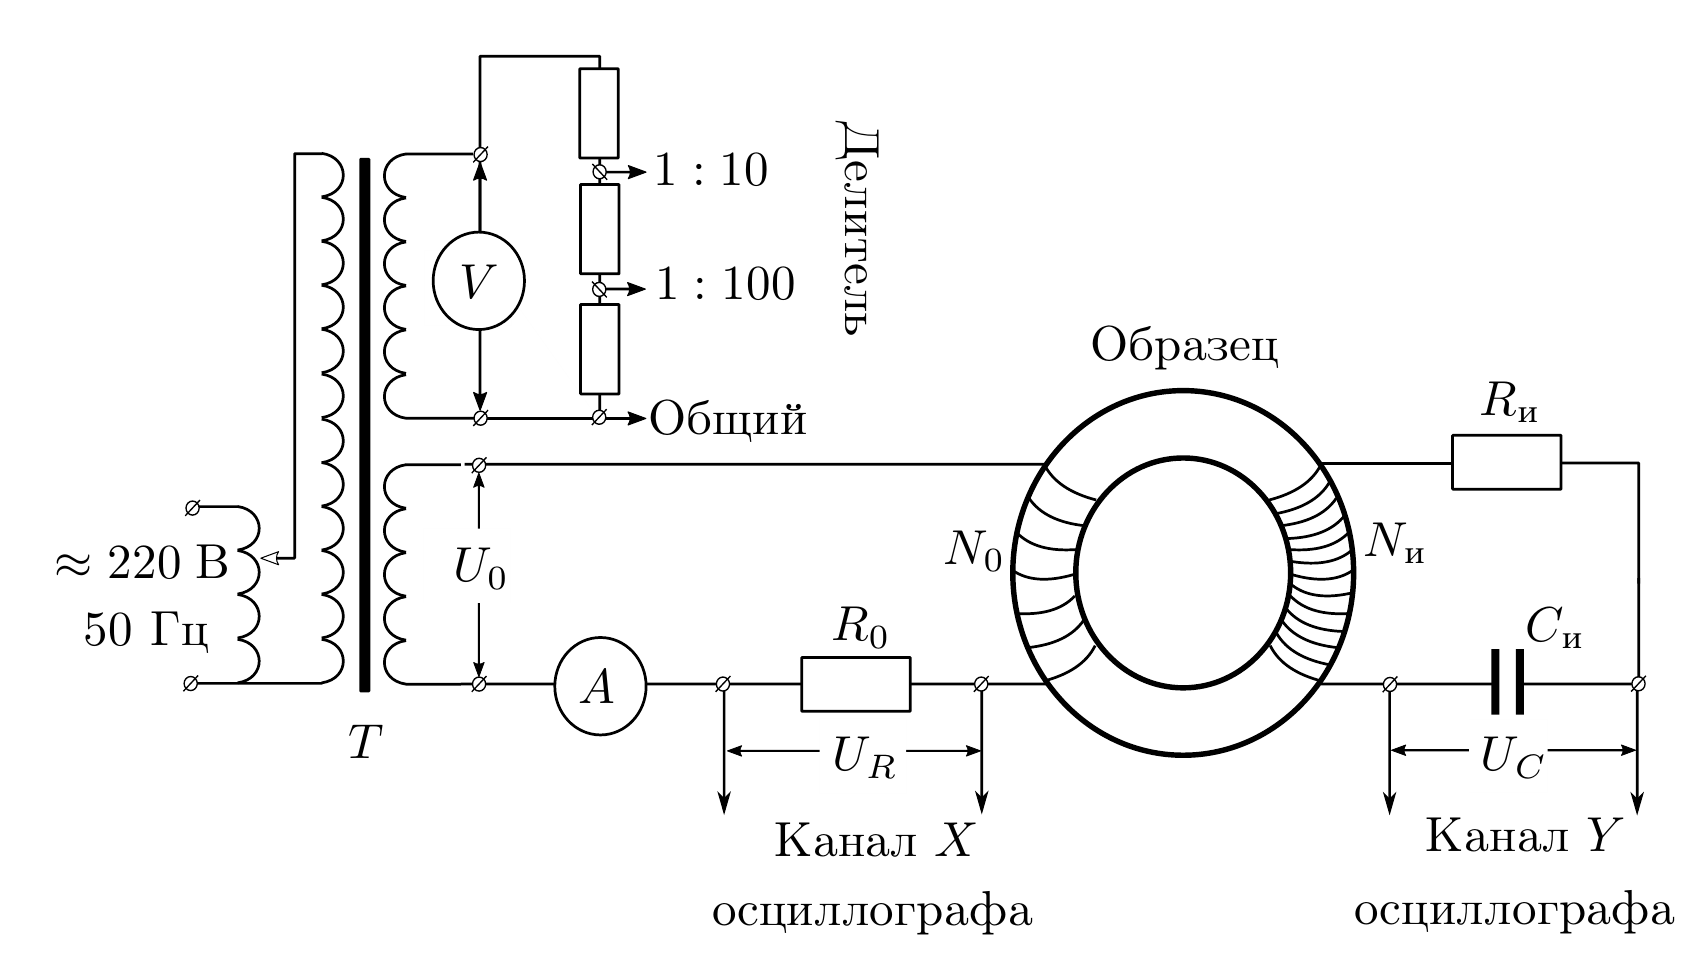
\includegraphics[scale=2]{3.png}
	\caption{ Схема установки для исследования намагничивания образцов}
	\label{fig:scheme}
\end{figure}

В цепь намагничивающей катушки, на которую подаётся некоторое
напряжение $U_0$, последовательно включено сопротивление $R_0$. Напряжение на $R_0$, равное $U_R = R_0I_0$, где $I_0$ — ток в намагничивающей обмотке $N_0$, подаётся на канал $ X $ осциллографа. Связь напряжённости $ H $ в
образце и тока $I_0$ рассчитывается по теореме о циркуляции. Действующее значение переменного тока в обмотке $N_0$ измеряется амперметром A. Для измерения магнитной индукции $ B $ с измерительной обмотки $N_\text{и}$ на вход $ RC $-цепочки подаётся напряжение $U_\text{и}$ ($U_{\text{вх}}$), пропорциональное производной $ dB/dt $. С интегрирующей ёмкости $C_\text{и}$ снимается напряжение $U_C$ ($U_{\text{вых}}$), пропорциональное величине $ B $, и подаётся на вход $ Y $ осциллографа. Значение индукции поля $ B $ рассчитывается по формуле \eqref{eq:|B|new}. Замкнутая кривая, возникающая на экране, воспроизводит в некотором масштабе (различном для осей $ X $ и $ Y $) петлю гистерезиса. Пример изображения предельной петли гистерезиса на осциллографе представлен на рис. \ref{fig:Perm:petlya}. Чтобы придать этой кривой количественный смысл, необходимо установить масштабы изображения, т. е. провести калибровку каналов $ X $ и $ Y $ осциллографа.

\begin{figure}[h]
\begin{center}
    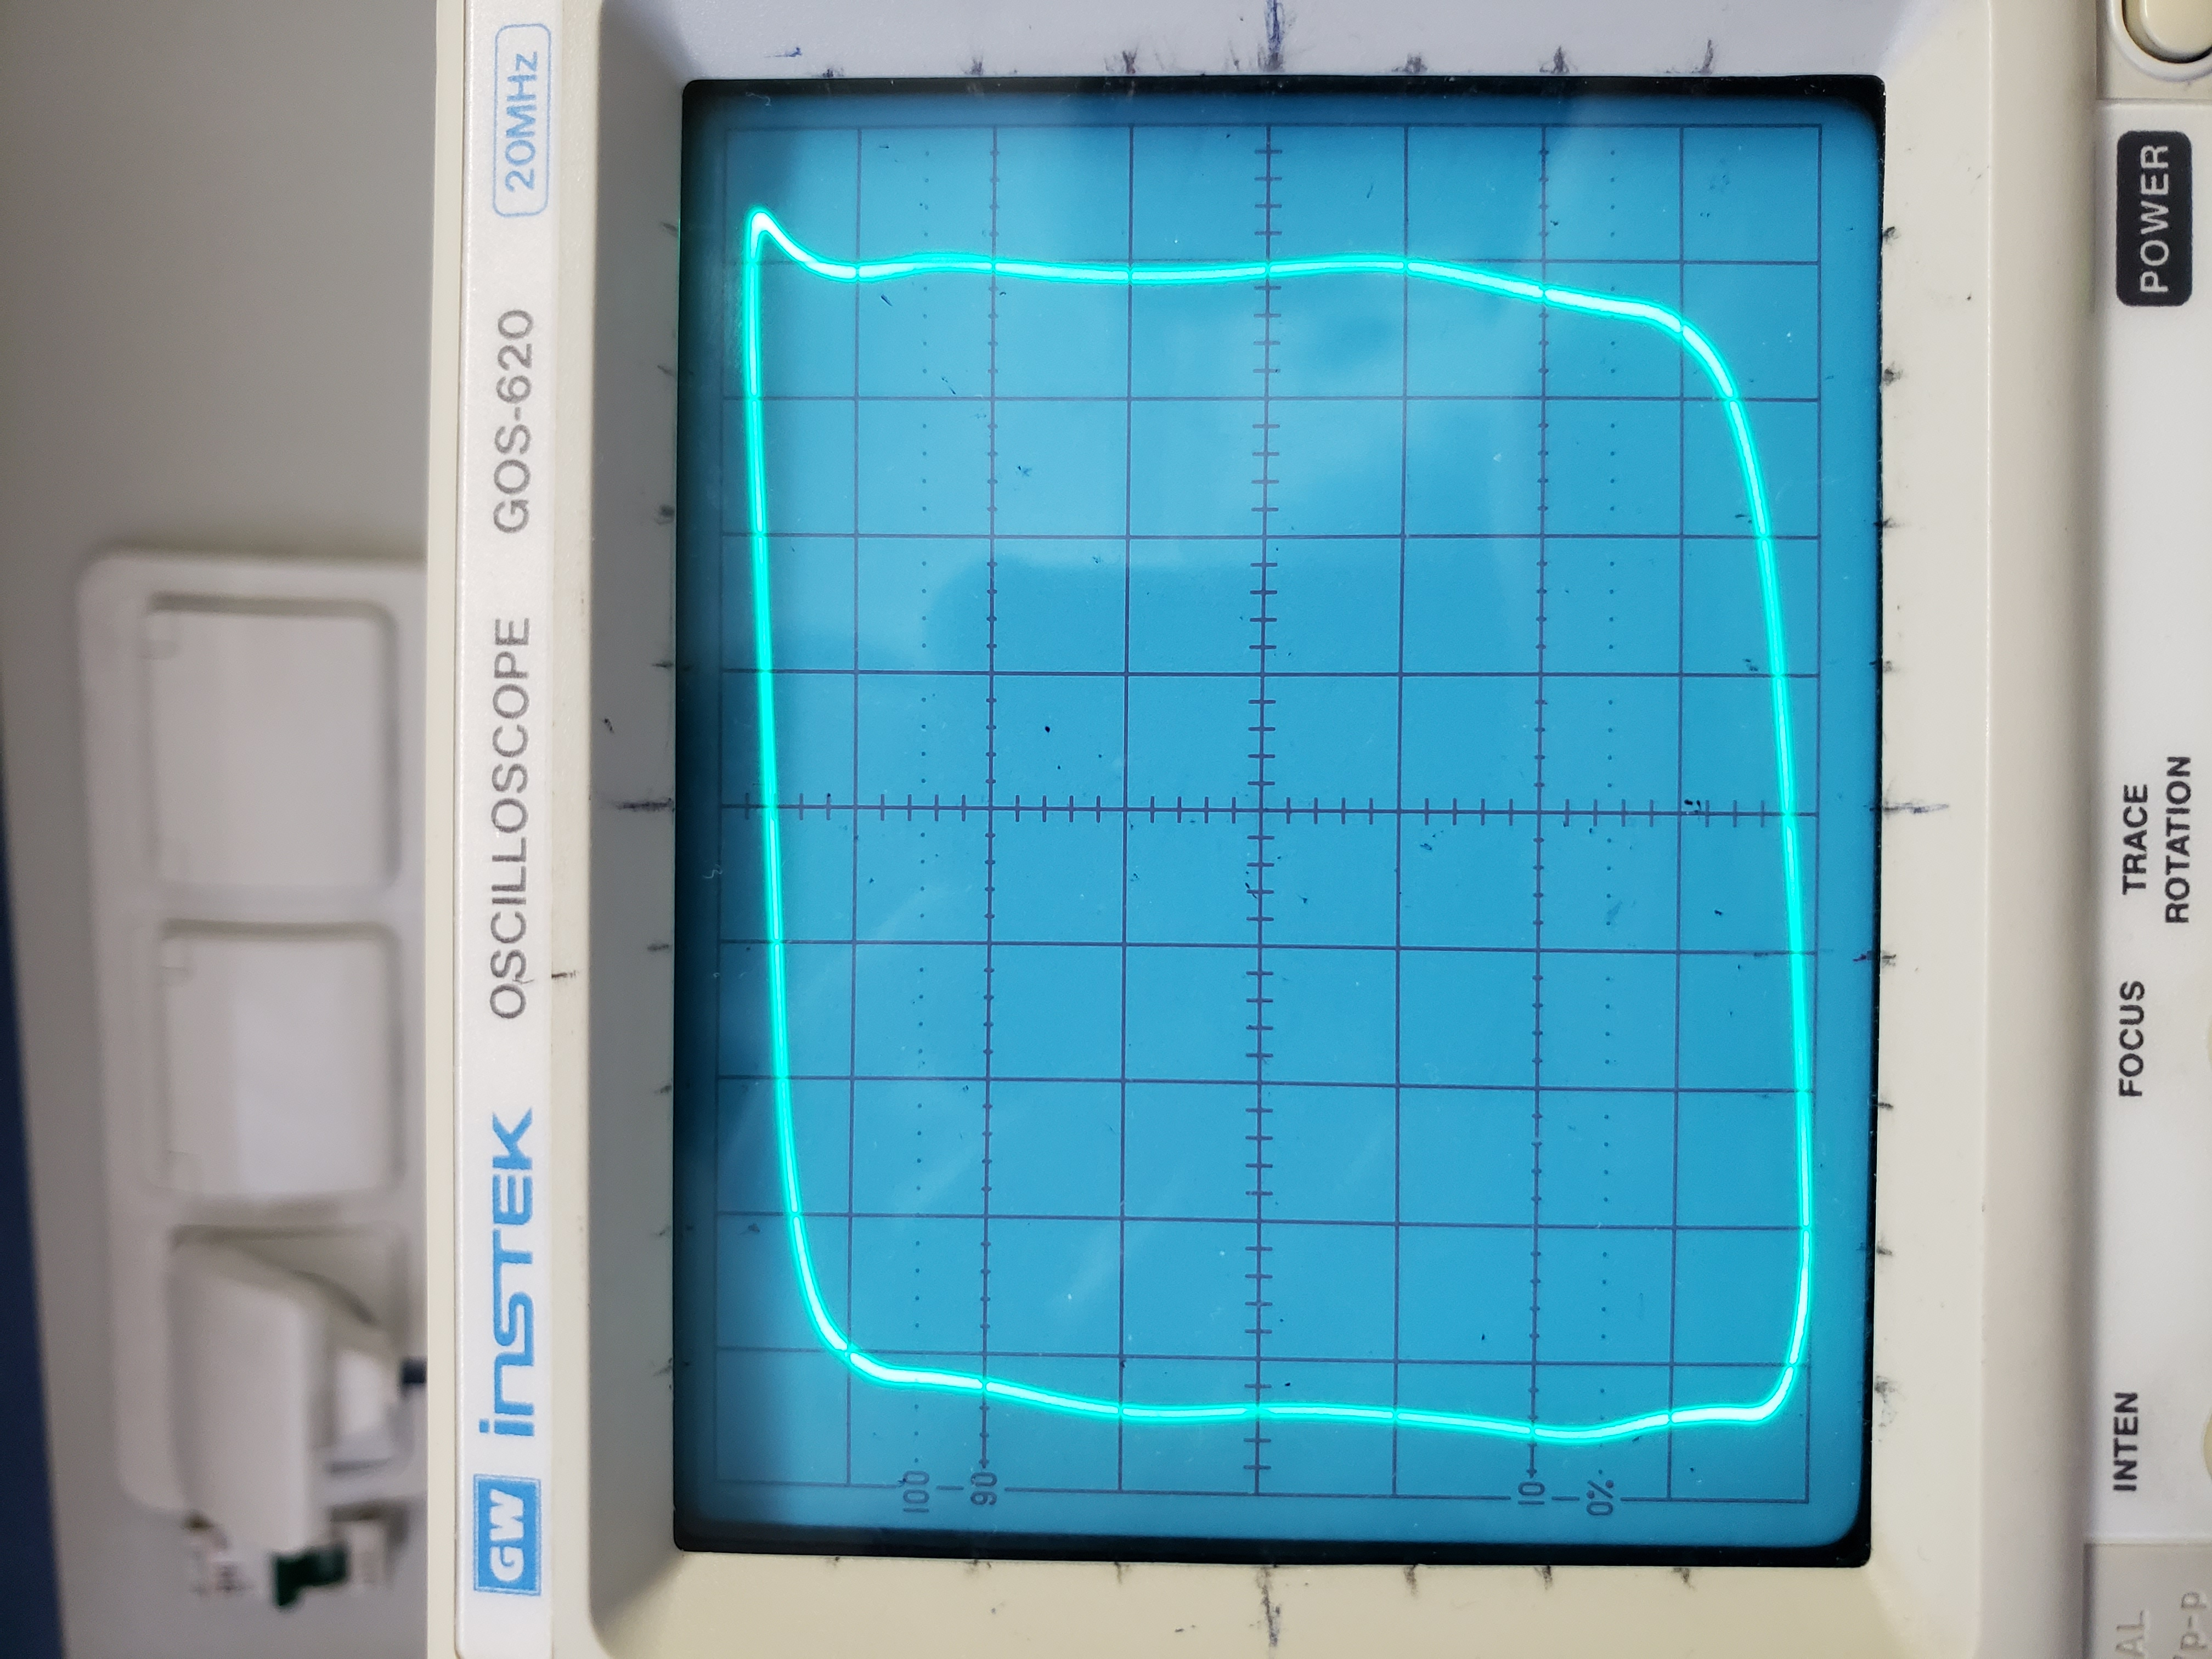
\includegraphics[width=0.4\textwidth]{perm.jpg}
\end{center}
\caption{Предельная петля гистерезиса пермаллоя}
\label{fig:Perm:petlya}
\end{figure}
  	
\section{Оборудование и инструментальные погрешности}

\textbf{В работе использовались:} автотрансформатор, понижающий трансформатор, интегрирующая цепочка, амперметр, вольтметр, электронный осциллограф, делитель напряжения, тороидальные образцы с двумя обмотками.

\textbf{Инструментальные погрешности:}
\begin{itemize}
    \item \textbf{Амперметр:} $\delta_U = \delta_I = 1\%$;
    \item \textbf{Осциллограф:} чувствительность осциллографа определяется в ходе работы для каждого значения масштаба.
\end{itemize}

\section{Результаты измерений и обработка экспериментальных данных}

Параметры установки: $R_0 = 0,2~Ом$, $R_и = 20~кОм$, $C_и = 20~мкФ$.

\begin{table}[h!]
\begin{center}
\begin{tabular}{|c|c|c|c|}
\hline 
 & Кремнистое железо & Пермаллой & Феррит \\ 
\hline 
$N_0$, витков & 20 & 15 & 45 \\ 
\hline 
$N_U$, витков & 200 & 300 & 400 \\ 
\hline 
$S$, $см^2$ & 2 & 0,66 & 3 \\ 
\hline 
$2\pi R$, $см$ & 11 & 14,1 & 25 \\ 
\hline 
\end{tabular} 
\end{center}
\caption{Характеристики исследуемых образцов}
\label{tab1}
\end{table}

Если известна чувствительность канала $K_x$ в [B/дел], то удвоенная амплитуда напряжения определяется произведением $$2U_{x_0} = 2x \cdot K_x.$$ Напряжение, подаваемое на вход Y определяется аналогично.

Калибровку осей осциллографа можно использовать для построения кривой гистерезиса в координатах $B$ и $H$. Зная величину сопротивления $R_0$, с которого снимается сигнал, можно определить чувствительность канала по току $K_{I_x} = \frac{K_x}{R_0}$ [A/дел], а затем по формуле

\begin{equation}\label{eq:H(del)}
H = \frac{I N_0}{2 \pi R} = \frac{K_x N_0}{2 \pi R R_0}
\end{equation}

определить цену деления шкалы в [А/м]. Используя формулу

\begin{equation}\label{eq:B(del)}
B = \frac{R_и C_и U_{вых}}{S N_U}
\end{equation}

можно рассчитать цену деления вертикальной шкалы в [Тл].

\newpage

\subsection{Кремнистое железо}

Измерения проводились при следующих параметрах: $K_x = 10~мВ/дел$, $K_y = 5~мВ/дел$, $I_{эф} = 141,4\pm1,4~мA$, $U = 4,96\pm0,01~B$. Результаты измерений:
\begin{description}
\item{} $2X_s = 87~мВ$
\item{} $2Y_s = 23~мВ$
\item{} $2X_c = 14~мВ$
\item{} $2Y_r = 19~мB$
\end{description}

По формулам \eqref{eq:H(del)} и \eqref{eq:B(del)} рассчитаем амплитуду $H_{max}$ колебаний напряжённости поля в тороиде, соответствующую состоянию насыщения (предельная петля), индукцию насыщения образца $B_s$, коэрцитивное поле $H_c$ и остаточную индукцию $B_r$. Полученные значения:

\begin{description}
\item{} $H_{max} = 581,8\pm9,1~А/м$
\item{} $B_s = 1,00\pm0,12~Тл$
\item{} $H_c = 86,4\pm0,5~А/м$
\item{} $B_r = 0,4\pm0,03~Тл$
\end{description}

Результаты измерения начальной кривой намагничивания представлены на графике~\ref{fig:Fe-Si:nach_petlya}.

\begin{figure}[h!]
\begin{center}
    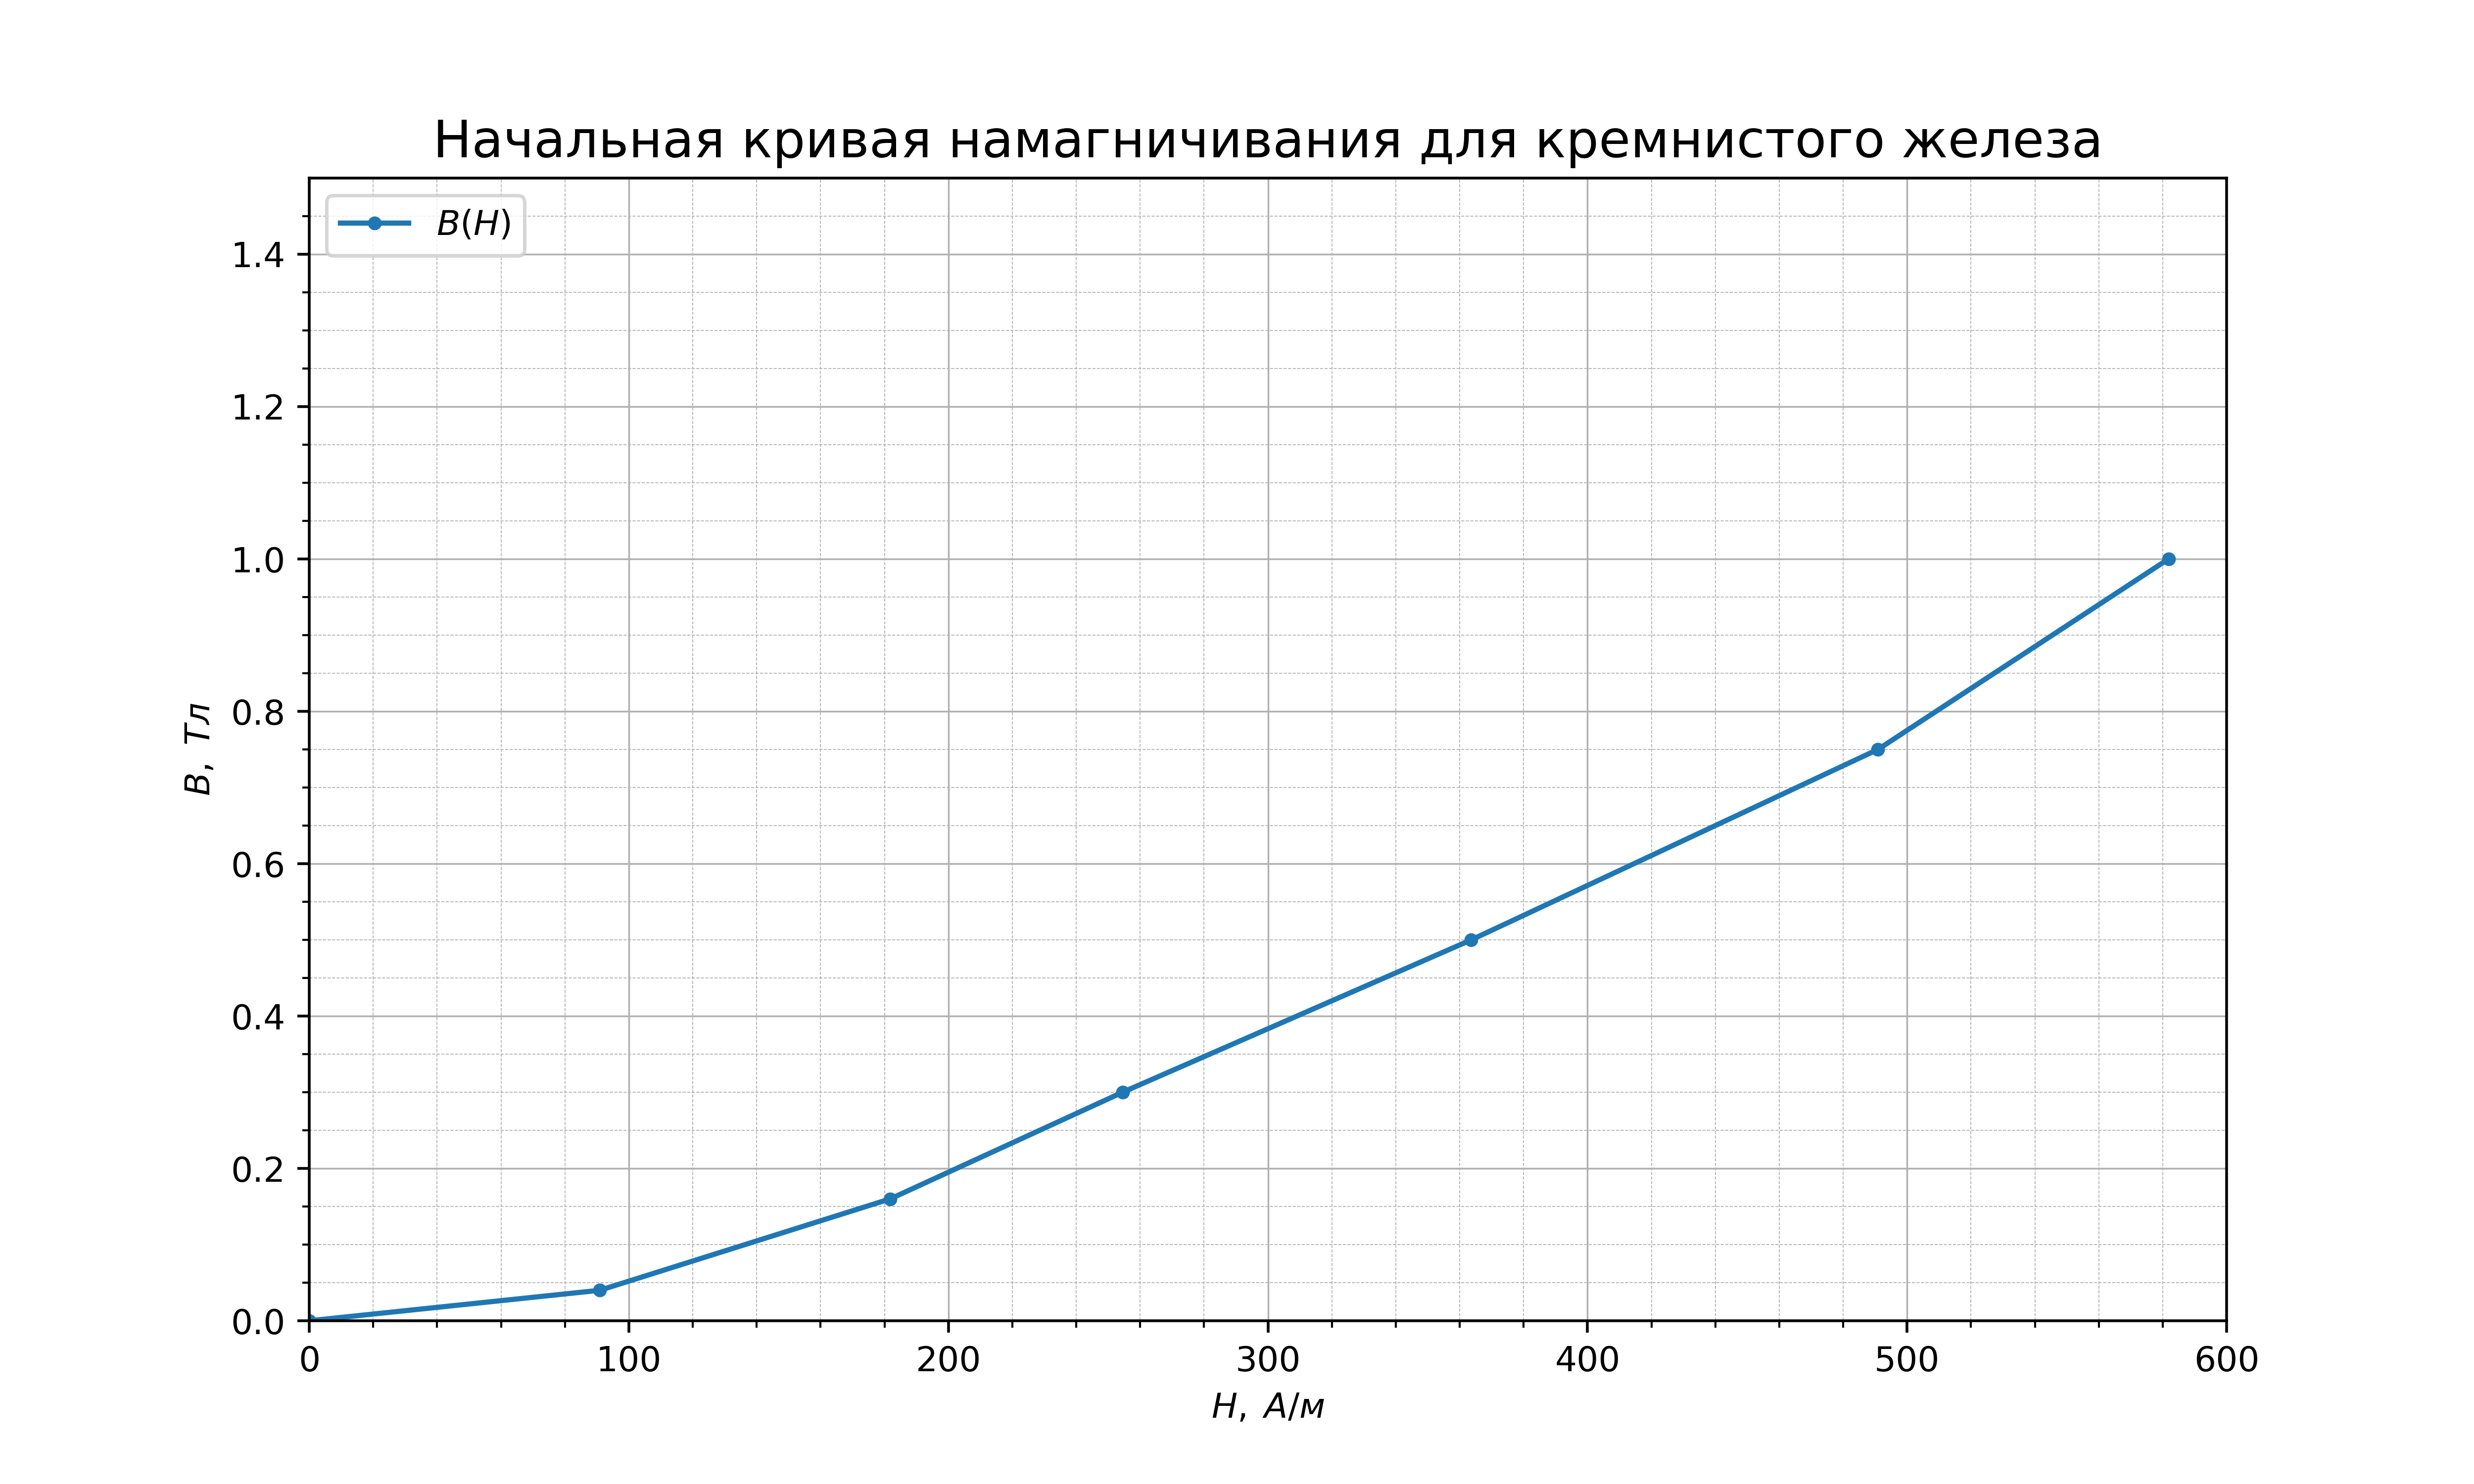
\includegraphics[scale=0.7]{3.4.5_1.png}
\end{center}
\caption{Начальная кривая намагничивания для кремнистого железа в координатах $B(H)$}
\label{fig:Fe-Si:nach_petlya}
\end{figure}

Начальное и максимальное значения дифференциальной магнитной проницаемости~$\mu_{диф}$ совпадают и равны $\mu_{диф} = 2500\pm300$.

\subsection{Пермаллой}

Измерения проводились при следующих параметрах: $K_x = 10~мВ/дел$, $K_y = 20~мВ/дел$, $I_{эф} = 168,3\pm1~мA$, $U = 5,13\pm0,01~B$. Результаты измерений:
\begin{description}
\item{} $2X_s = 90\pm10~мВ$
\item{} $2Y_s = 160\pm10~мВ$
\item{} $2X_c = 84\pm5~мВ$
\item{} $2Y_r = 152\pm10~мB$
\end{description}

По формулам \eqref{eq:H(del)} и \eqref{eq:B(del)} рассчитаем амплитуду $H_{max}$ колебаний напряжённости поля в тороиде, соответствующую состоянию насыщения (предельная петля), индукцию насыщения образца $B_s$, коэрцитивное поле $H_c$ и остаточную индукцию $B_r$. Полученные значения:
\begin{description}
\item{} $H_{max} = 30,6\pm2,6~А/м$
\item{} $B_s = 1,8\pm0,1~Тл$
\item{} $H_c = 28,9\pm2,5~А/м$
\item{} $B_r = 1,7\pm0,1~Тл$
\end{description}

Результаты измерения начальной кривой намагничивания представлены на графике~\ref{fig:Perm:nach_petlya}.

\begin{figure}[h!]
\begin{center}
    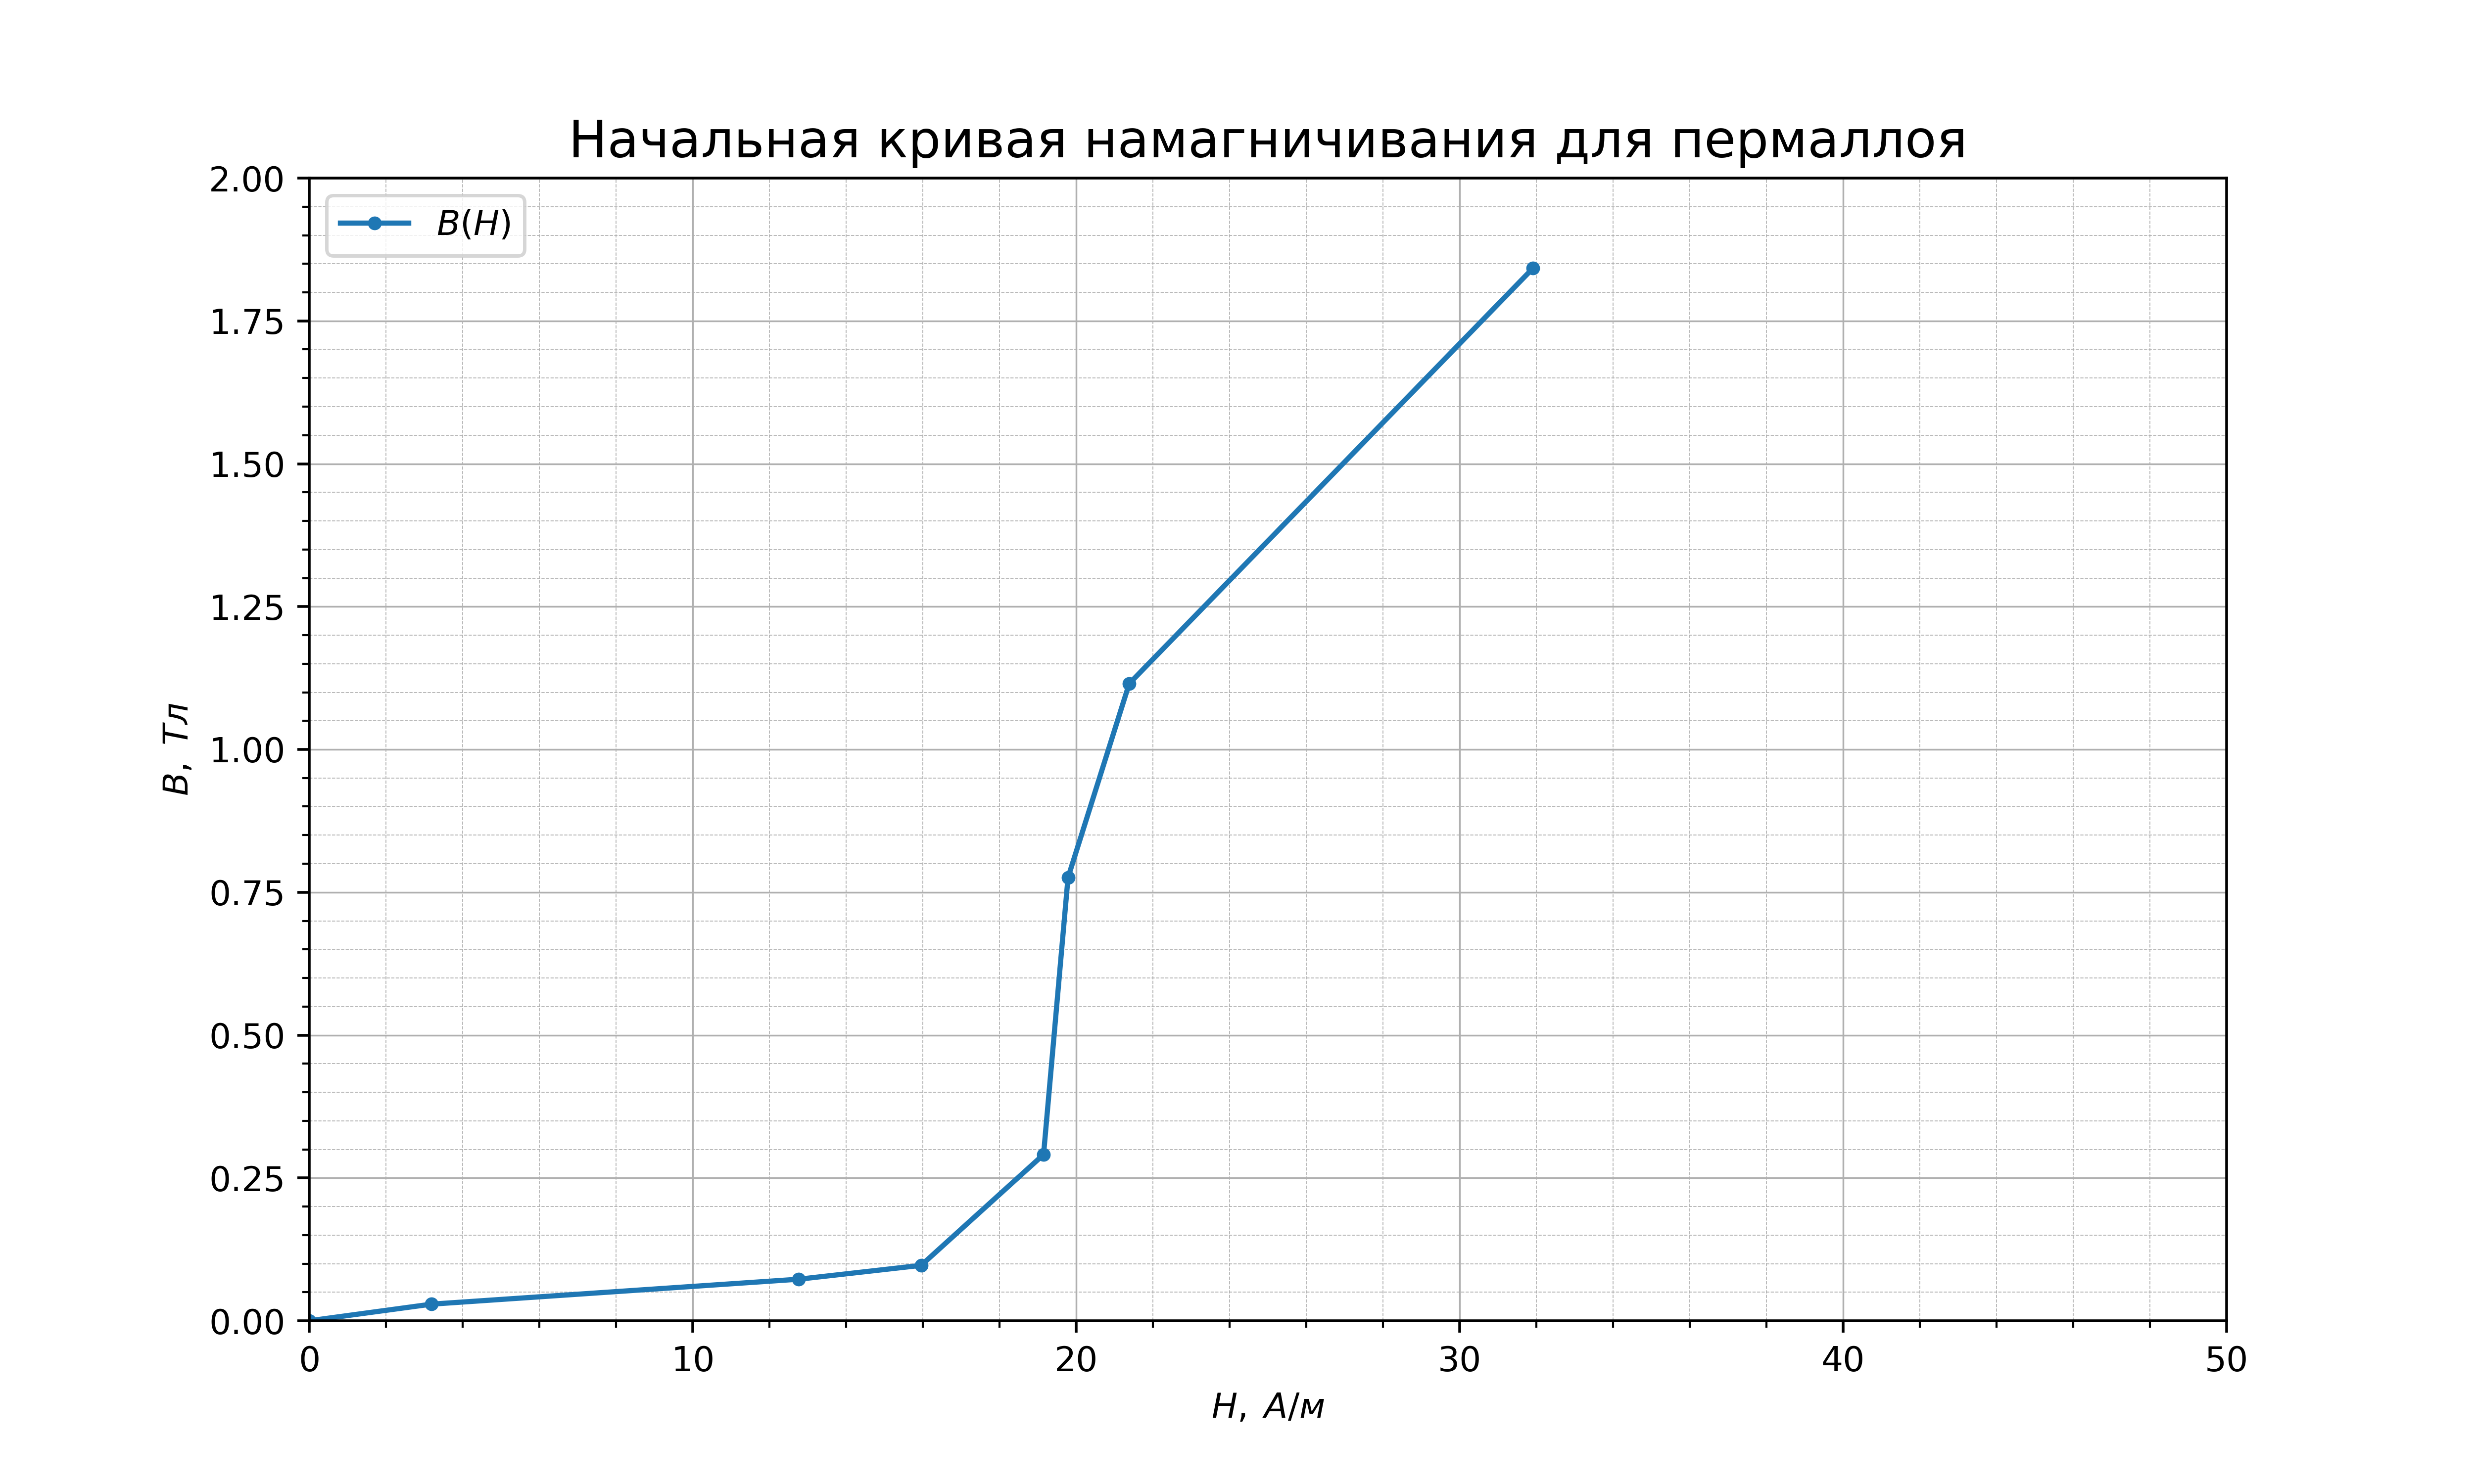
\includegraphics[scale=0.7]{3.4.5_2.png}
\end{center}
\caption{Начальная кривая намагничивания для пермаллоя в координатах $B(H)$}
\label{fig:Perm:nach_petlya}
\end{figure}

Начальное значение дифференциальной магнитной проницаемости \newline $\mu_{диф} = 30000\pm5000$. Максимальное значение равно $\mu_{диф} = 334225\pm60000$.

\subsection{Феррит}

Измерения проводились при следующих параметрах: $K_x = 5~мВ/дел$, $K_y = 5~мВ/дел$, $I_{эф} = 27\pm1~мA$, $U = 5,11\pm0,01~B$. Результаты измерений:
\begin{description}
\item{} $2X_s = 15\pm10~мВ$
\item{} $2Y_s = 25\pm5~мВ$
\item{} $2X_c = 10\pm2~мВ$
\item{} $2Y_r = 14,5\pm5~мB$
\end{description}

По формулам \eqref{eq:H(del)} и \eqref{eq:B(del)} рассчитаем амплитуду $H_{max}$ колебаний напряжённости поля в тороиде, соответствующую состоянию насыщения (предельная петля), индукцию насыщения образца $B_s$, коэрцитивное поле $H_c$ и остаточную индукцию $B_r$. Полученные значения:
\begin{description}
\item{} $H_{max} = 45,0\pm4,5~А/м$
\item{} $B_s = 0,16\pm0,01~Тл$
\item{} $H_c = 30,0\pm0,9~А/м$
\item{} $B_r = 0,09\pm0,01~Тл$
\end{description}

Результаты измерения начальной кривой намагничивания представлены на графике~\ref{fig:Ferrit:nach_petlya}.

\begin{figure}[h!]
\begin{center}
    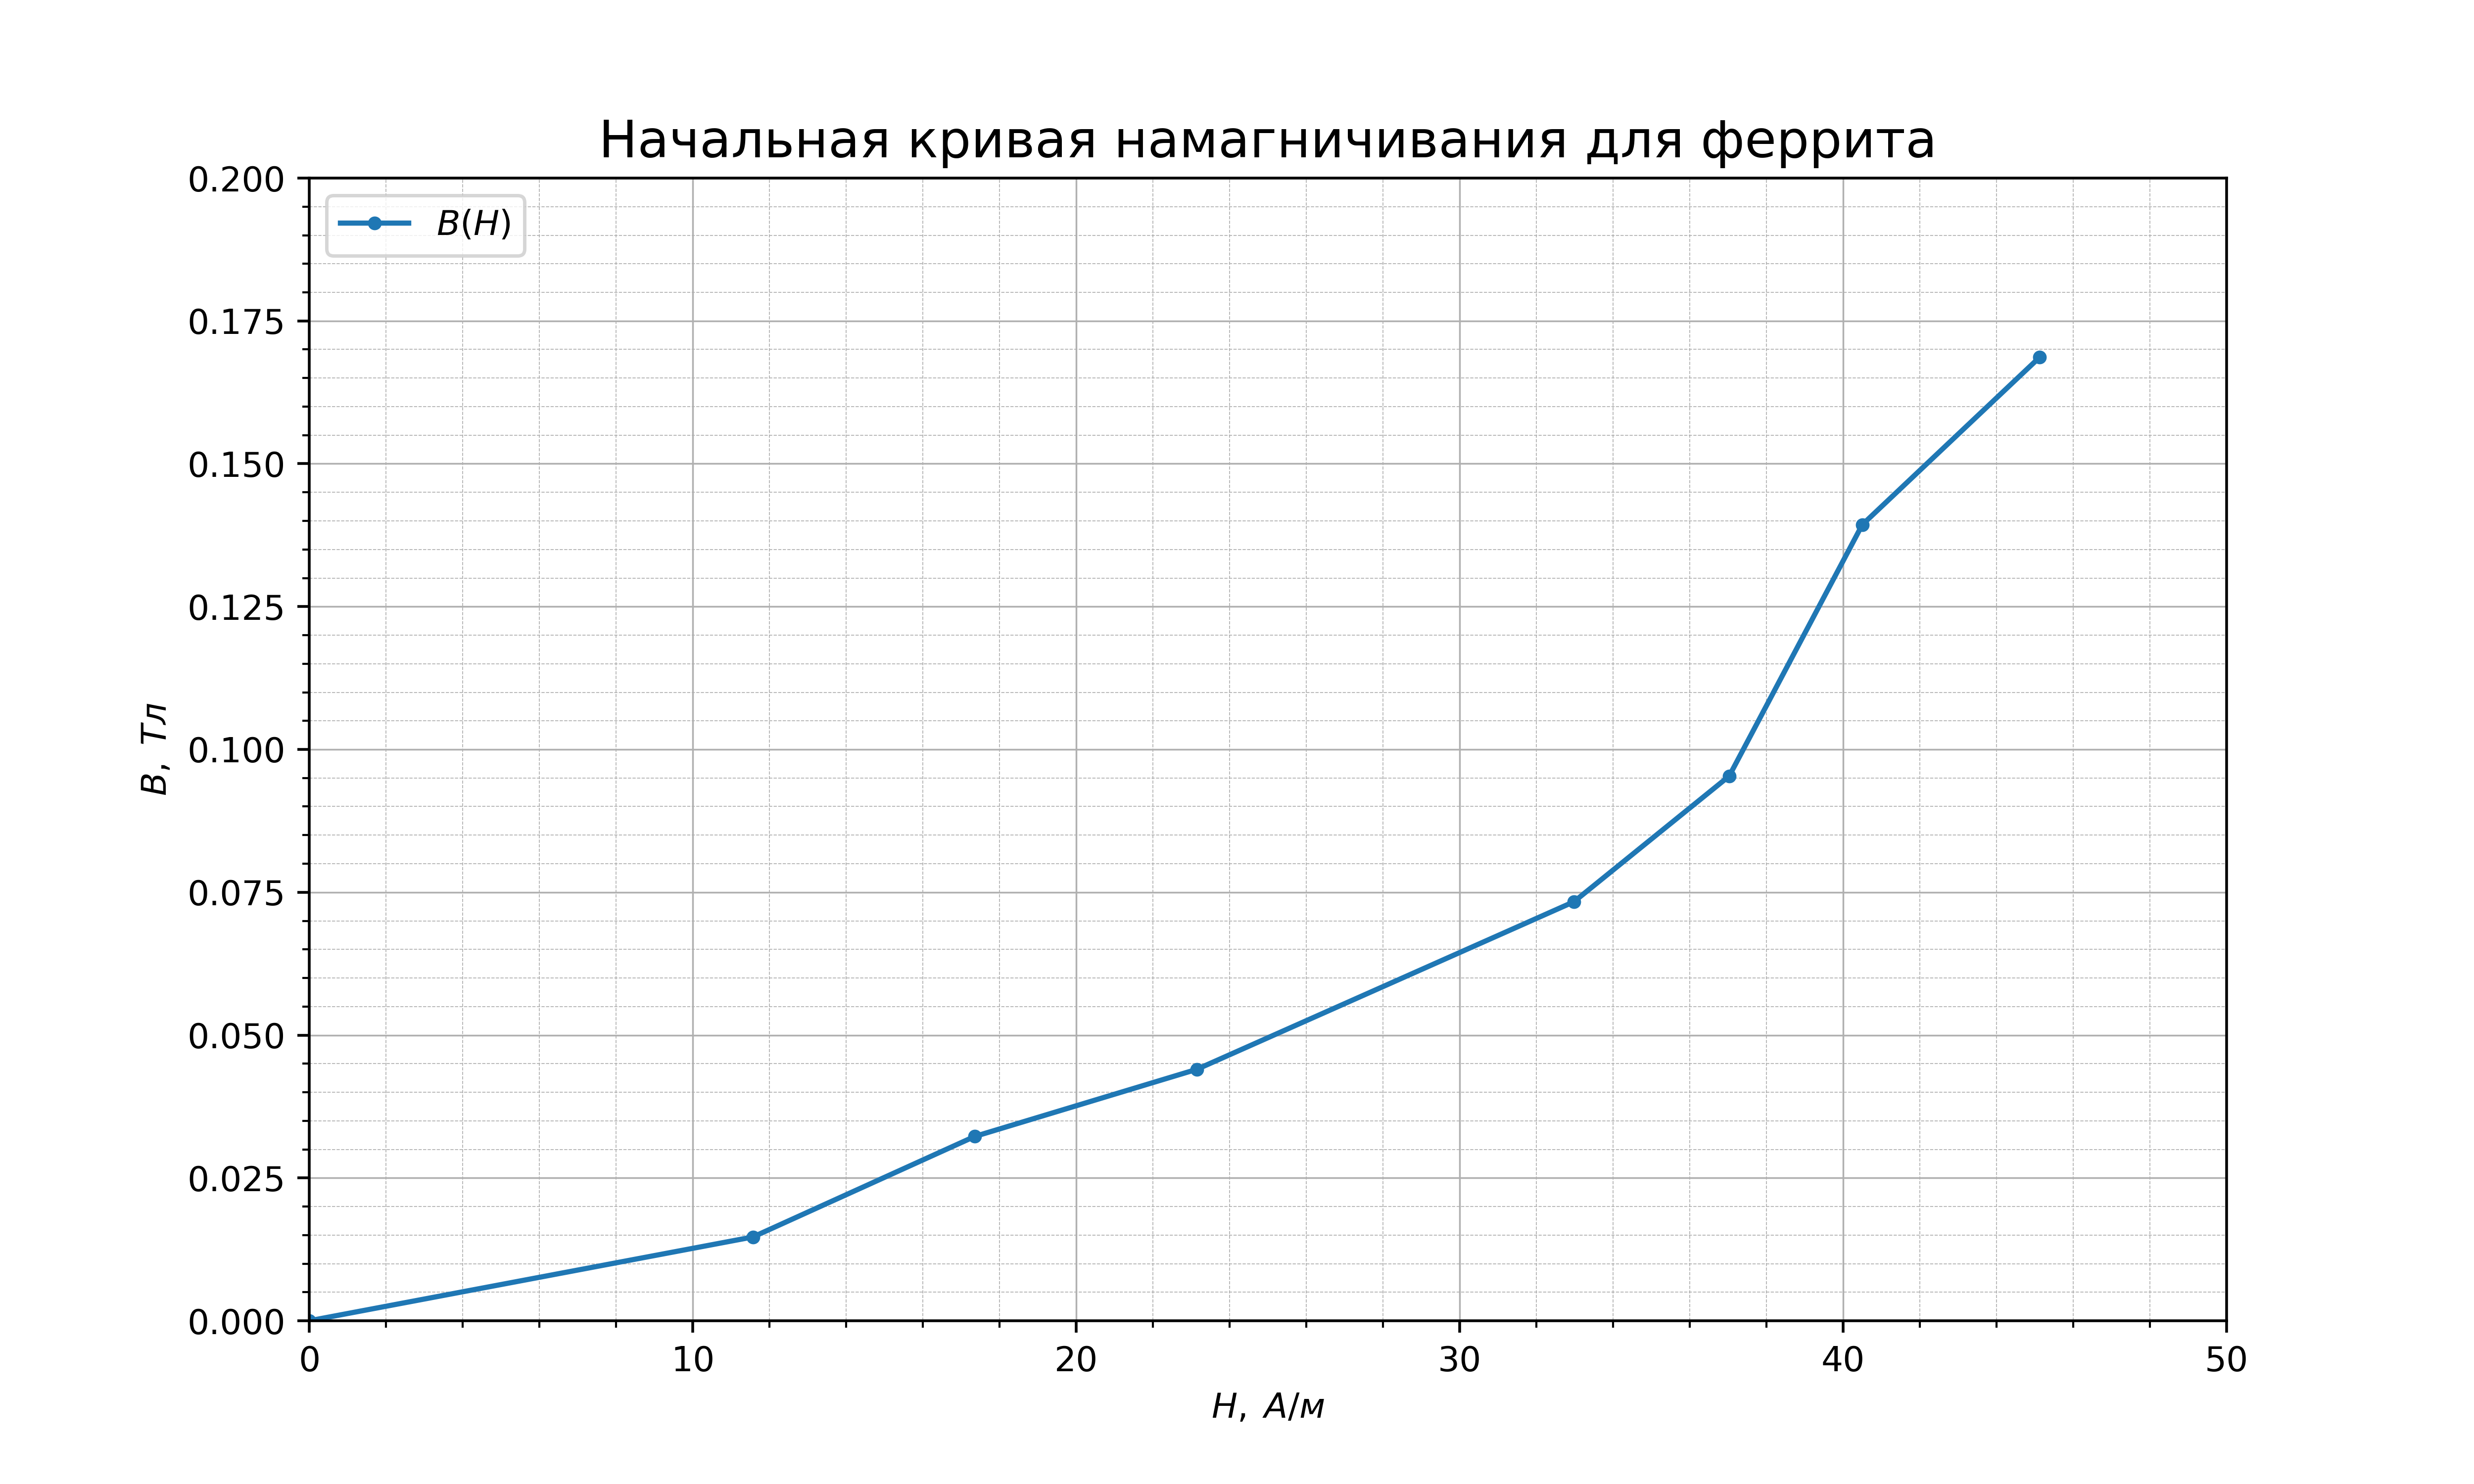
\includegraphics[scale=0.7]{3.4.5_3.png}
\end{center}
\caption{Начальная кривая намагничивания для феррита в координатах $B(H)$}
\label{fig:Ferrit:nach_petlya}
\end{figure}

Начальное и максимальное значения дифференциальной магнитной проницаемости~$\mu_{диф}$ совпадают и равны $\mu_{диф} = 6000\pm500$.

\newpage

\subsection{Проверка калибровки осциллографа}

Для $K_x = 5~мВ/дел$:
$$m_x = \frac{2\sqrt{2} \cdot 0,2  \cdot 0,086}{10} = 48,6\pm0,5~мВ/дел.$$

Для $K_x = 10~мВ/дел$:
$$m_x = \frac{2\sqrt{2} \cdot 0,2  \cdot 0,102}{6} = 9,8\pm0,1~В/дел.$$

Для $K_y = 20~мВ/дел$:
$$m_y = 2\sqrt{2} \cdot \frac{U_{эф}}{2y} = \frac{2\sqrt{2} \cdot 0,054}{8} = 19\pm1~мВ/дел.$$

Для $K_y = 5~мВ/дел$:
$$m_y = \frac{2\sqrt{2} \cdot 0,01}{6} = 4,95\pm0,05~мВ/дел.$$

Калибровка выполнена с достаточной точностью.

\subsection{Определение параметров $RC$-ячейки}

С помощью формул \eqref{eq:tauone} и \eqref{eq:tautwo} определим теоретически и экспериментально значение $\tau_c$

\begin{description}
\item{} $K_x = 1~В/дел$, $x = 4,5\pm1~дел$, $U_{вх} = 2x \cdot K_x = 9\pm2~В$;
\item{} $K_y = 5~мВ/дел$, $y = 7\pm1~дел$, $U_{вых} = 2y \cdot K_y = 0,07\pm0,013~В$.
\end{description}

$$\tau_{эксп} = \frac{U_{вх}}{\omega U_{вых}} = 0,42\pm0,05~с.$$

$$\tau_{теор} = R_и C_и = 0,4~с.$$

\newpage

\section{Обсуждение результатов и выводы}

В данной работе были исследованы предельные петли гистерезиса и начальные кривые намагничивания для 3 ферромагнитных образцов. Были определены магнитные характеристики материалов, а также некоторые параметры установки. Результаты измерений в сравнении с табличными значениями представлены в таб.~\ref{tab2}.

\begin{table}[h!]
\begin{center}
\begin{tabular}{|c|c|c|c|c|}
\hline
 & Ампл. & Кремнистое железо & Пермаллой & Феррит \\ \hline
эксп & \multirow{2}{*}{$H_c$, A/м} & $86,4 \pm 0,5$ & $28,9 \pm 2,5$ & $30,0 \pm 0,9$ \\ \cline{1-1} \cline{3-5} 
табл &  & 100 & 11--40 & 20 \\ \hline
эксп & \multirow{2}{*}{$B_s$, Тл} & $1 \pm 0,12$ & $1,8 \pm 0,1$ & $0,16 \pm 0,01$ \\ \cline{1-1} \cline{3-5} 
табл &  & 2 & 1,5 & 0,15 \\ \hline
эксп & \multirow{2}{*}{$\mu_{диф}$} & $2500 \pm 300$ & $30000 \pm 5000$ & $6000 \pm 500$ \\ \cline{1-1} \cline{3-5} 
табл &  & 20000 & 8000--35000 & 10000 \\ \hline
\end{tabular}
\end{center}
\caption{Сравнение полученных значений с табличными}
\label{tab2}
\end{table}

Многие полученные значения существенно отличаются от табличных. Это может быть связано с несовершенством методики измерений, а также расположением элементов установки друг относительно друга. Например, очень большие отклонения полученных значений $\mu_{диф}$ могут быть связаны с невозможностью достаточно точно промерить кривую намагничивания. Однако, удалось оценочно определить некоторые магнитные параметры и получить примерные кривые намагничивания.

Также в данной работе была проверена калибровка осциллографа и определена постоянная времени $\tau$ $RC$-цепочки. По результатам измерений было получено, что калибровка осциллографа выполнена с достаточной точностью. Значение $\tau$, рассчитанное экспериментально, согласуется с рассчитанным теоретически в рамках погрешности. 

\textbf{Выводы:} в ходе данной работы удалось экспериментально гистерезиса для нескольких образцов ферромагнетиков. Были вычислены верные по порядку значения магнитной проницаемости, коэрцитивного поля и остаточной индукции для материалов образцов. Проверено, что осциллограф даёт достаточную точность для измерения параметров петли гистерезиса. Установлено, что применённая в работе экспериментальная установка даёт недостаточную точность для количественного измерения характеристик ферромагнетиков, но даёт качественно пронаблюдать явление гистерезиса.

\end{document}